% !TEX root = ../ApproxDA-TransUNet.tex
\section{Optimization Dynamics and Routing Mechanics}
\label{sec:optimization_routing}
\label{sec:generalization}

Having established how Semantic Spatial Dependency governs segmentation accuracy across tasks, we now examine the microscopic behavior of ApproxDA-TransUNet: how windowed approximation alters late-stage training dynamics (Section~\ref{sec:volatility}), and why learnable dual-branch attention gates collapse to uniform routing (Section~\ref{sec:collapse}).

\subsection{Windowed Attention as a Task-Dependent Regularizer}
\label{sec:volatility}

To investigate how spatial approximation affects the training landscape, we analyze optimization trajectories across representative datasets spanning the GCS spectrum (Synapse for high GCS; Kvasir-SEG and ISIC 2018 for low GCS). We define \emph{validation DSC volatility} as the standard deviation of validation DSC evaluated at 15-epoch intervals over the final 30\% of training (epochs~210--300, 7 evaluation checkpoints). Low volatility signifies smooth, stable convergence near the optimum, while high volatility indicates oscillatory optimization.

Table~\ref{tab:volatility} summarizes best validation DSC, test DSC, generalization gap ($\text{Val} - \text{Test}$), and late-stage volatility for DA-TransUNet and ApproxDA-TransUNet.

\begin{table*}[tb]
  \caption{Optimization Volatility and Generalization Gap across Representative Benchmarks Spanning the GCS Spectrum. Volatility is measured as the standard deviation of validation DSC over epochs 210--300 (lower is more stable).}
  \label{tab:volatility}
  \centering
  \setlength{\tabcolsep}{6pt}
  \begin{tabular}{llccccc}
    \toprule
    Dataset & GCS Tier & Model Architecture & Best Val (\%) & Test DSC (\%) & Val$-$Test Gap & Volatility ($\sigma_\text{val}$) \\
    \midrule
    Synapse  & High & DA-TransUNet          & 79.52 & 79.80 & $-$0.28 & 0.409 \\
    Synapse  & High & ApproxDA ($M{=}28$)   & 81.02 & 80.94 & $+$0.08 & 0.542 \\
    \midrule
    Kvasir-SEG & Low  & DA-TransUNet          & 88.38 & 88.44 & $-$0.06 & 0.769 \\
    Kvasir-SEG & Low  & ApproxDA ($M{=}7$)    & 89.23 & 89.24 & $-$0.01 & \textbf{0.042} ($18.2\times$ reduction) \\
    \midrule
    ISIC 2018  & Low  & DA-TransUNet          & 87.71 & 88.43 & $-$0.72 & 0.479 \\
    ISIC 2018  & Low  & ApproxDA ($M{=}7$)    & 89.56 & 89.58 & $-$0.02 & \textbf{0.053} ($9.0\times$ reduction) \\
    \bottomrule
  \end{tabular}
\end{table*}

\begin{figure*}[tb]
  \centering
  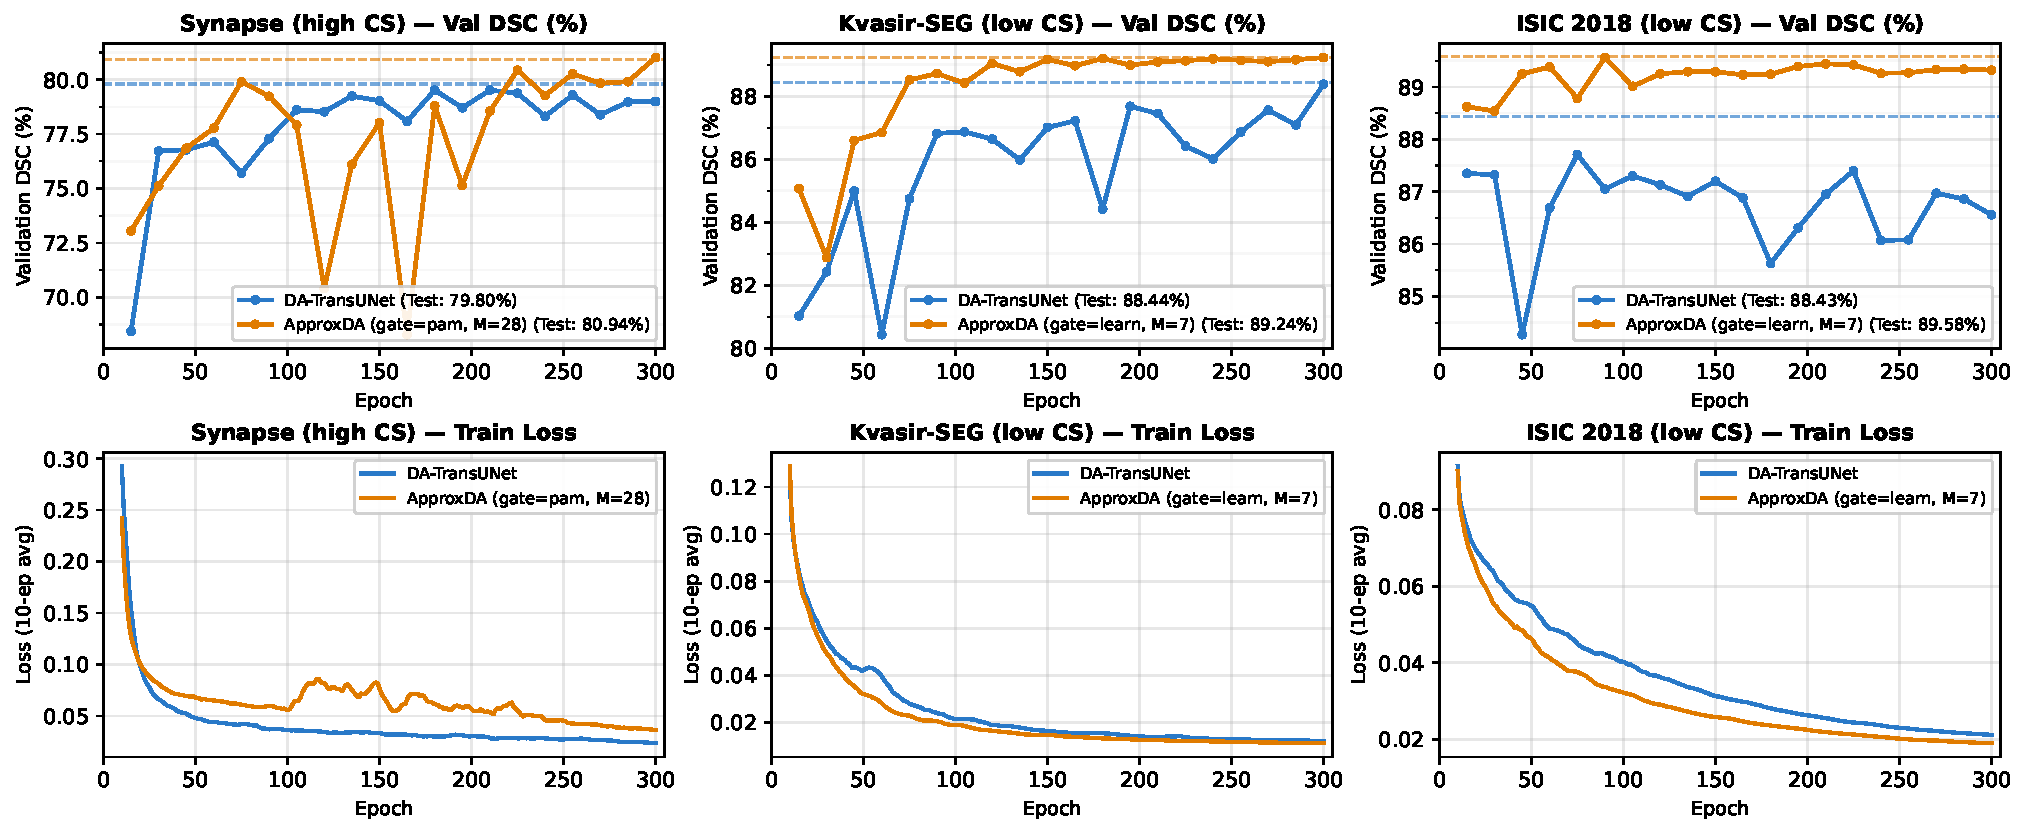
\includegraphics[width=\textwidth]{figures/fig_f1_generalization_gap.pdf}
  \caption{Optimization trajectories for DA-TransUNet (blue) vs.\ ApproxDA-TransUNet (orange). Top row: Validation DSC trajectories across epochs (dashed lines indicate final test DSC). Bottom row: Corresponding training loss trajectories (10-epoch rolling averages).}
  \label{fig:generalization}
\end{figure*}

\textbf{GCS-dependent volatility crossover.} As illustrated in Figure~\ref{fig:generalization}, tracking validation DSC and training loss reveals a striking, task-dependent crossover:
\begin{itemize}
  \item \textbf{Low-GCS stabilization:} On low-GCS tasks, ApproxDA-TransUNet dramatically stabilizes late-stage training, reducing validation volatility by $18.2\times$ on Kvasir-SEG (0.042 vs.\ 0.769) and $9.0\times$ on ISIC 2018 (0.053 vs.\ 0.479).
  \item \textbf{High-GCS inversion:} On high-GCS Synapse, this stability advantage reverses: ApproxDA-TransUNet exhibits $1.3\times$ higher volatility than DA-TransUNet (0.542 vs.\ 0.409).
\end{itemize}

This crossover provides direct dynamic evidence for the locality inductive bias hypothesis: on low-GCS tasks where local boundary cues dominate, windowed attention suppresses noisy long-range gradient signals originating from irrelevant tissue, acting as an \emph{implicit regularizer} that smooths the late-stage optimization landscape. Conversely, on high-GCS Synapse where multi-organ co-localization is essential, windowing restricts cross-organ gradient flow, creating tension between local feature extraction and global organ balance that manifests as higher optimization volatility.

Furthermore, across all evaluated settings, the generalization gap remains tight ($\le 0.72\%$), with test performance closely tracking validation scores. This confirms that the observed volatility reduction is a fundamental characteristic of the optimization dynamics rather than an artifact of overfitting.

\subsection{Gate Dynamics and Gradient Symmetry Collapse}
\label{sec:collapse}

We next investigate the routing dynamics between spatial (PAM) and channel (CAM) attention branches. While learnable scalar gates are widely utilized in dual-branch architectures to adaptively balance representations, empirical evaluations show that learned gating frequently underperforms fixed routing.

Table~\ref{tab:gate_ablation} compares gate configurations on Synapse ($M{=}7$, $r{=}32$). Fixed spatial attention (gate=pam, 78.64\% DSC) consistently outperforms CAM-only (78.26\%) and both learnable gate configurations (77.78\% at $M{=}7$; 78.04\% at $M{=}14$, $r{=}64$).

\begin{table}[ht]
  \caption{Gate Mode Ablation on Synapse ($M$=7, $r$=32)}
  \label{tab:gate_ablation}
  \centering
  \setlength{\tabcolsep}{5pt}
  \small
  \begin{tabular}{llcc}
    \toprule
    Gate Mode & $g$ & DSC (\%) $\uparrow$ & HD95 (mm) $\downarrow$ \\
    \midrule
    gate=pam                    & 1.0              & \textbf{78.64} & 31.09 \\
    gate=cam                    & 0.0              & \underline{78.26}  & \underline{30.59} \\
    gate=learn ($M$=14, $r$=64) & ${\approx}0.5^*$ & 78.04          & \textbf{29.09} \\
    gate=learn                  & ${\approx}0.5^*$ & 77.78          & 34.29 \\
    \bottomrule
  \end{tabular}
  \par\vspace{5pt}
  \parbox{\columnwidth}{\footnotesize $^*$Gate collapsed to $g{\approx}0.5$ throughout training.}
\end{table}

\begin{figure}[tbp]
  \centering
  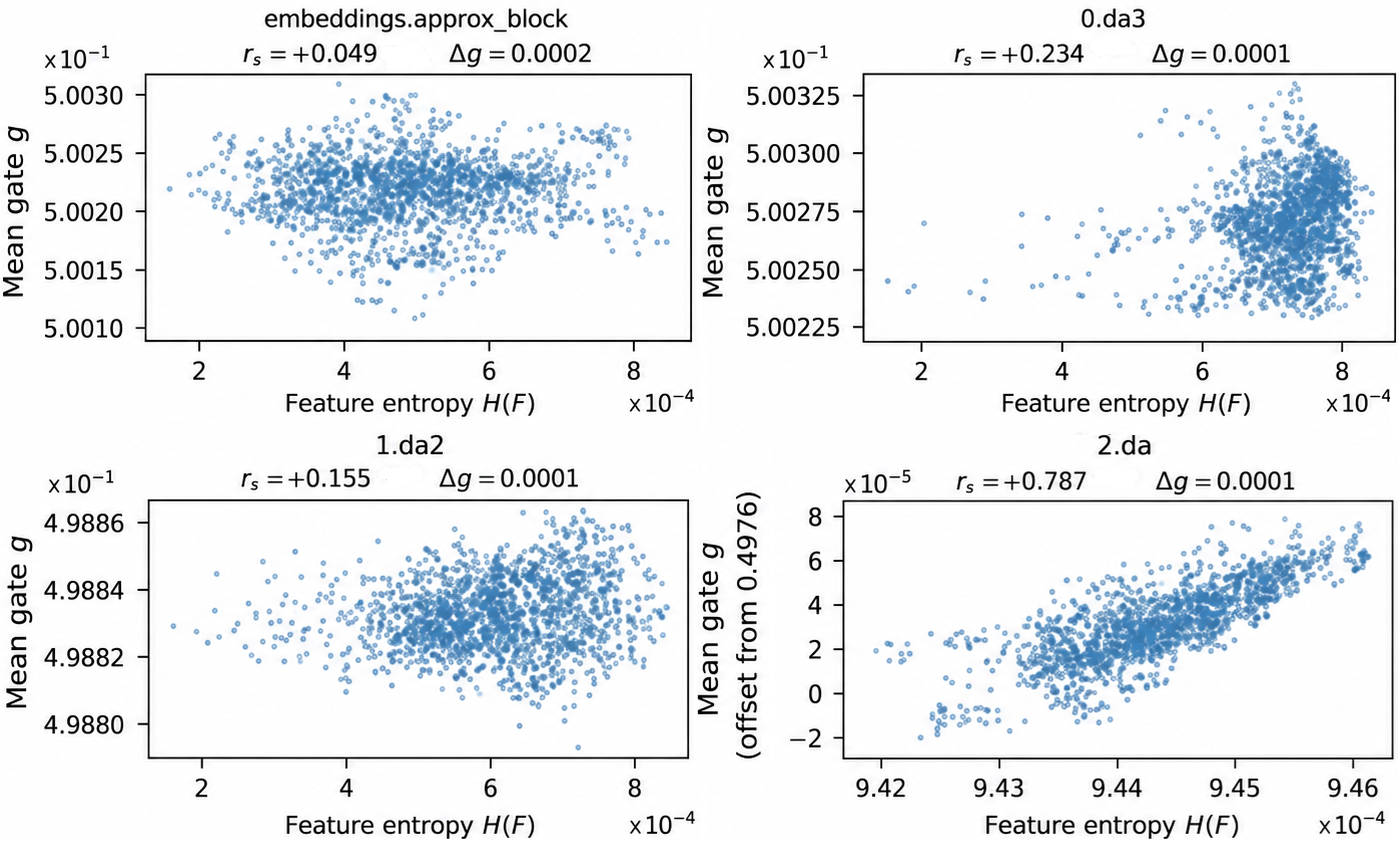
\includegraphics[width=\columnwidth]{figures/fig_entropy_scatter.png}
  \caption{Learned gate value $g$ vs.\ input feature entropy $H(F)$ across all four network depths ($M{=}7$, gate=learn). Gate values cluster at $g \approx 0.5$ ($\Delta g \le 0.0002$) with zero correlation to entropy ($r_s \approx 0$).}
  \label{fig:gate_analysis}
\end{figure}

\textbf{Mathematical derivation of gate collapse.} Given the fused feature representation $\mathbf{F} = g \mathbf{F}_\text{P} + (1-g) \mathbf{F}_\text{C}$, the analytic gradient with respect to gate parameter $g$ is:
\begin{equation}
  \frac{\partial\mathcal{L}}{\partial g} = \frac{\partial\mathcal{L}}{\partial\mathbf{F}} \cdot \left(\mathbf{F}_\text{P} - \mathbf{F}_\text{C}\right).
  \label{eq:gate_grad}
\end{equation}
At standard initialization ($g \approx 0.5$), the backpropagated gradients into both PAM and CAM branches are symmetric:
\begin{equation}
  \frac{\partial\mathcal{L}}{\partial\mathbf{F}_\text{P}} = g \frac{\partial\mathcal{L}}{\partial\mathbf{F}} \approx \frac{1}{2}\frac{\partial\mathcal{L}}{\partial\mathbf{F}}, \qquad \frac{\partial\mathcal{L}}{\partial\mathbf{F}_\text{C}} = (1-g)\frac{\partial\mathcal{L}}{\partial\mathbf{F}} \approx \frac{1}{2}\frac{\partial\mathcal{L}}{\partial\mathbf{F}}.
\end{equation}
Because both branches receive identical supervision without structural asymmetry or branch-specialization incentives, the learned representations rapidly converge toward mutual similarity ($\mathbf{F}_\text{P} \approx \mathbf{F}_\text{C}$). Consequently, the differential term $(\mathbf{F}_\text{P} - \mathbf{F}_\text{C})$ vanishes, forcing $\partial\mathcal{L}/\partial g \approx 0$. This establishes a self-reinforcing stable equilibrium that locks $g$ at $\approx 0.5$ throughout optimization.

\textbf{Empirical verification across stages.} As depicted in Figure~\ref{fig:gate_analysis}, tracking learned gate values against feature entropy across all four network stages (bottleneck, $28^2$, $56^2$, $112^2$) reveals that gate values stay pinned at $g = 0.5000 \pm 0.0002$, with Spearman rank correlation $r_s \approx 0$. This demonstrates that the gate fails to adapt to input complexity.

These findings show that conventional scalar gating in symmetric dual-branch architectures cannot achieve adaptive routing. Effective multi-branch transformer architectures must either employ fixed, task-aligned routing (e.g., gate=pam) or introduce explicit structural asymmetries and diversity-promoting objective functions.
